\documentclass[11pt,a4paper,landscape]{article}
\usepackage[margin=0.65in]{geometry}
\usepackage{xcolor}
\usepackage{titlesec}
\usepackage{enumitem}
\usepackage{booktabs}
\usepackage{array}
\usepackage{tabularx}
\usepackage{tikz}
\usetikzlibrary{arrows.meta,positioning,shapes.geometric,fit}

\definecolor{sarthiGreen}{HTML}{5B7051}
\definecolor{sarthiInk}{HTML}{1F241E}
\definecolor{sarthiMuted}{HTML}{687367}
\definecolor{sarthiSoft}{HTML}{F4F7F1}
\definecolor{sarthiLine}{HTML}{D7DFD1}
\definecolor{sarthiGold}{HTML}{C69A42}

\titleformat{\section}{\Large\bfseries\color{sarthiGreen}}{}{0em}{}
\titleformat{\subsection}{\normalsize\bfseries\color{sarthiInk}}{}{0em}{}
\setlist[itemize]{leftmargin=1.2em,itemsep=0.18em,topsep=0.2em}
\setlist[enumerate]{leftmargin=1.4em,itemsep=0.18em,topsep=0.2em}
\renewcommand{\arraystretch}{1.2}

\newcommand{\tagline}[1]{\vspace{0.25em}\noindent\textcolor{sarthiMuted}{#1}\vspace{0.6em}}
\newcommand{\pill}[1]{\colorbox{sarthiSoft}{\strut\hspace{0.45em}#1\hspace{0.45em}}}

\tikzset{
  box/.style={rectangle, rounded corners=5pt, draw=sarthiLine, fill=white, align=center, minimum height=8mm, text width=28mm, font=\small},
  widebox/.style={rectangle, rounded corners=5pt, draw=sarthiLine, fill=white, align=center, minimum height=8mm, text width=38mm, font=\small},
  db/.style={cylinder, cylinder uses custom fill, cylinder body fill=sarthiSoft, cylinder end fill=sarthiSoft, shape border rotate=90, aspect=0.28, draw=sarthiGreen, align=center, text width=26mm, minimum height=11mm, font=\small},
  decision/.style={diamond, draw=sarthiGold, fill=white, align=center, aspect=2.1, text width=24mm, inner sep=1pt, font=\small},
  arrow/.style={-Latex, thick, draw=sarthiGreen},
  softarrow/.style={-Latex, draw=sarthiMuted}
}

\begin{document}

\begin{center}
{\Huge\bfseries\color{sarthiGreen} Sarthi}\\[0.35em]
{\Large Product Plan and High-Level Flow}\\[0.7em]
{\large Trust assistant for confident checkout decisions}\\[1.1em]
\pill{Buyer trust} \quad \pill{Seller improvement} \quad \pill{Admin governance} \quad \pill{Checkout confidence}
\end{center}

\vspace{0.8em}

\section{1. Product Goal}
Sarthi helps a buyer answer one practical question before placing an order:

\begin{center}
\fcolorbox{sarthiLine}{sarthiSoft}{\parbox{0.86\linewidth}{\centering\large
\textbf{Can I trust this product, this seller, this size, this offer, and this payment choice before checkout?}}}
\end{center}

The goal is to reduce wrong purchases, avoidable returns, and COD rejection by giving the buyer a simple evidence-backed decision before checkout.

\section{2. Problem}
Buyers often struggle because:
\begin{itemize}
  \item many sellers list similar-looking products;
  \item the cheapest option may not be the safest;
  \item seller rating and product rating can conflict;
  \item size, fabric, color, and quality are hard to judge online;
  \item reviews may be generic, misleading, or not relevant to the exact SKU;
  \item offer timers and prepaid offers can create pressure;
  \item COD rejection causes delivery cost, return cost, inventory lock, support load, and seller loss.
\end{itemize}

Sarthi solves this by checking evidence before recommendation instead of making the buyer guess.

\section{3. Users}
\begin{tabularx}{\linewidth}{>{\bfseries}p{0.18\linewidth}X}
\toprule
Buyer & Needs a simple recommendation, size help, offer truth, payment confidence, and privacy control.\\
Seller & Needs fair discovery, clear improvement tasks, and aggregate buyer feedback without seeing private buyer data.\\
Admin / Reviewer & Needs control over seller verification, listing approval, proof review, and auditability.\\
\bottomrule
\end{tabularx}

\section{4. Product Surfaces}
Sarthi has three connected surfaces:
\begin{enumerate}
  \item Buyer App
  \item Seller Portal
  \item Admin Review Console
\end{enumerate}

All three use the same trust evidence layer: product and SKU facts, seller verification, seller and product ratings, review credibility, return reasons, price and offer history, payment offers, buyer fit memory, seller proof assets, order outcomes, and audit traces.

\section{5. Core Buyer Experience}
\begin{enumerate}
  \item Buyer searches, opens, or wishlists a product.
  \item Sarthi checks if similar seller listings exist.
  \item Sarthi calculates a trust score for the product-SKU-seller combination.
  \item Buyer sees a simple recommendation, reason, size guidance, and warning.
  \item Buyer can ask Sarthi a product question.
  \item If proof is missing, Sarthi creates an aggregate seller proof request.
  \item At checkout, Sarthi checks offer truth and whether prepaid can be safely nudged.
  \item Buyer chooses COD or prepaid.
  \item Delivery outcome updates future trust.
\end{enumerate}

\section{6. Core Features}
\begin{tabularx}{\linewidth}{>{\bfseries}p{0.24\linewidth}X}
\toprule
Feature & Purpose\\
\midrule
Trust Score & Shows a score like 72/100 with confidence, reason breakdown, risks, and missing evidence.\\
Similar Listing Resolver & Compares similar products from different sellers and recommends one safer option plus one alternative.\\
New Seller Fair-Start & Gives verified new sellers fair exposure while keeping buyer confidence provisional.\\
Per-SKU Trust Passport & Shows trust for the exact variant, including proof, return reasons, and missing evidence.\\
Size Oracle & Recommends the safest size using buyer memory and SKU/category outcomes.\\
Galti Mat Dohrao & Shows one avoidable warning such as color mismatch, fabric risk, or size risk.\\
Sarthi Samvaad & Lets buyer ask natural questions about fit, fabric, seller trust, offer, and checkout.\\
Knowledge Graph & Connects seller, product, SKU, reviews, returns, proof, offer, checkout, and outcomes.\\
Review Credibility & Downweights generic, repeated, stale, or contradicted reviews.\\
Checkout Confidence & Nudges prepaid only when product, seller, offer, refund, and delivery trust are strong enough.\\
Seller Evidence Coach & Converts buyer doubts into aggregate seller proof and improvement tasks.\\
Admin Review & Controls seller verification, listing approval, proof validation, and audit trail.\\
\bottomrule
\end{tabularx}

\section{7. Trust Score Approach}
The trust score is not a random AI number. It is calculated from weighted evidence:

\begin{tabularx}{\linewidth}{>{\bfseries}p{0.34\linewidth}X}
\toprule
Attribute & Why it matters\\
\midrule
SKU kept-order outcome & Real kept/returned behavior is the strongest signal.\\
Seller reliability and verification & Seller behavior affects fulfillment, support, and trust.\\
Fit and size consistency & Size mismatch is a major avoidable return reason.\\
Review credibility & Reviews matter only if relevant and believable.\\
Product rating quality & Product quality must be separate from seller rating.\\
Proof coverage & Proof reduces fabric, color, and packaging doubts.\\
Offer truth and dispatch & Important near checkout, but should not override product trust.\\
Price value & Price matters, but cheapest should not automatically win.\\
\bottomrule
\end{tabularx}

\tagline{Every score should show score, confidence, top positive reasons, top risks, evidence strength, and missing evidence.}

\section{8. New Seller Fair-Start}
New sellers should not start at zero trust only because they have fewer orders. Sarthi will use:
\begin{itemize}
  \item category prior for new listings;
  \item fair-start exposure for verified new sellers;
  \item confidence cap until enough outcomes exist;
  \item score adjustment as buyers keep or return products.
\end{itemize}

\begin{center}
\fcolorbox{sarthiLine}{sarthiSoft}{\parbox{0.82\linewidth}{\centering
\textbf{Fair-start improves opportunity, not fake buyer trust.}}}
\end{center}

\section{9. Knowledge Graph}
The graph connects:
\begin{center}
\texttt{Buyer -> Fit Memory -> SKU -> Product -> Seller -> Reviews -> Returns -> Proof -> Offer -> Checkout -> Outcome}
\end{center}

It helps answer why a seller is safer, whether ratings conflict, whether reviews are contradicted by returns, what proof is missing, and whether prepaid should be nudged at checkout.

\section{10. Review And Rating Logic}
\begin{tabularx}{\linewidth}{>{\bfseries}p{0.34\linewidth}X}
\toprule
Case & Handling\\
\midrule
Low seller rating, high product rating & Product may be good, but seller reliability remains risky.\\
High seller rating, low product rating & Seller may be reliable, but this SKU has quality, size, or fabric issues.\\
Positive reviews, high returns & Reviews may be false positives or irrelevant; contradicted attributes are downweighted.\\
\bottomrule
\end{tabularx}

\section{11. Checkout Confidence}
Sarthi nudges prepaid only when trust is strong enough.

\begin{tabularx}{\linewidth}{>{\bfseries}p{0.23\linewidth}p{0.28\linewidth}X}
\toprule
Mode & When & Buyer Copy\\
\midrule
Prepaid Recommended & Trust is strong and saving is verified. & Pay online to save Rs 40. Sarthi checked seller trust, product evidence, and offer truth. COD is still available.\\
Balanced Choice & Trust is moderate or proof is missing. & Prepaid can save Rs 25, but fabric proof is still limited. Choose prepaid only if you are comfortable.\\
No Prepaid Nudge & Trust is weak or data is unclear. & Sarthi is not recommending prepaid for this item yet because evidence is limited.\\
\bottomrule
\end{tabularx}

\tagline{Hard blockers: seller restricted, seller verification pending, offer not verified, weak product evidence, unclear refund/payment information, stale data, or high return risk.}

\section{12. Seller And Admin}
\textbf{Seller flow:} seller applies, gets verified, creates listing draft, receives aggregate proof tasks, submits proof or fixes listing details, and improves future buyer trust.

\vspace{0.35em}
\textbf{Admin flow:} admin controls seller approval, listing approval, proof review, revisions, and audit logs. This prevents sellers from self-declaring trust.

\section{13. Agentic AI Role}
Sarthi's AI is an orchestrator, not just a chatbot. It understands buyer intent, selects tools, checks facts, calculates or fetches trust score, verifies checkout confidence, creates seller proof requests when evidence is missing, gives a grounded answer, stores audit trace, and uses cache when facts have not changed.

\section{14. Data And Architecture}
\begin{tabularx}{\linewidth}{>{\bfseries}p{0.25\linewidth}X}
\toprule
Component & Purpose\\
\midrule
MongoDB Atlas & Stores product evidence, scores, traces, checkout sessions, proof requests, and cache.\\
Atlas Search & Searches products, reviews, seller proof, and text evidence.\\
Atlas Vector Search & Finds similar reviews, doubts, questions, and proof evidence.\\
Neo4j & Stores weighted relationships for graph reasoning.\\
Object Storage & Stores proof images, seller documents, and listing media.\\
\bottomrule
\end{tabularx}

\section{15. Implementation Phases}
\begin{enumerate}
  \item Trust Score: weighted score, breakdown, confidence, and new seller fair-start.
  \item Knowledge Graph: seller, product, SKU, reviews, returns, proof, offer, checkout, and outcome relationships.
  \item Checkout Confidence: prepaid confidence score and safe nudges.
  \item Seller Evidence Loop: buyer doubts and return reasons become aggregate seller tasks.
  \item MongoDB Atlas Integration: evidence, snapshots, traces, sessions, and cache.
  \item End-to-End Demo: connected buyer, checkout, seller, admin, and outcome learning flow.
\end{enumerate}

\section{16. Success Metrics}
\begin{itemize}
  \item kept-order rate;
  \item avoidable return reduction;
  \item COD rejection reduction;
  \item prepaid adoption under high-trust conditions;
  \item seller proof task completion;
  \item recommendation abstention when evidence is weak;
  \item cache hit rate for repeated agent queries;
  \item buyer memory opt-out correctness.
\end{itemize}

\newpage
\section{17. High-Level Flowcharts}

\subsection{17.1 Closed-Loop System}
\begin{center}
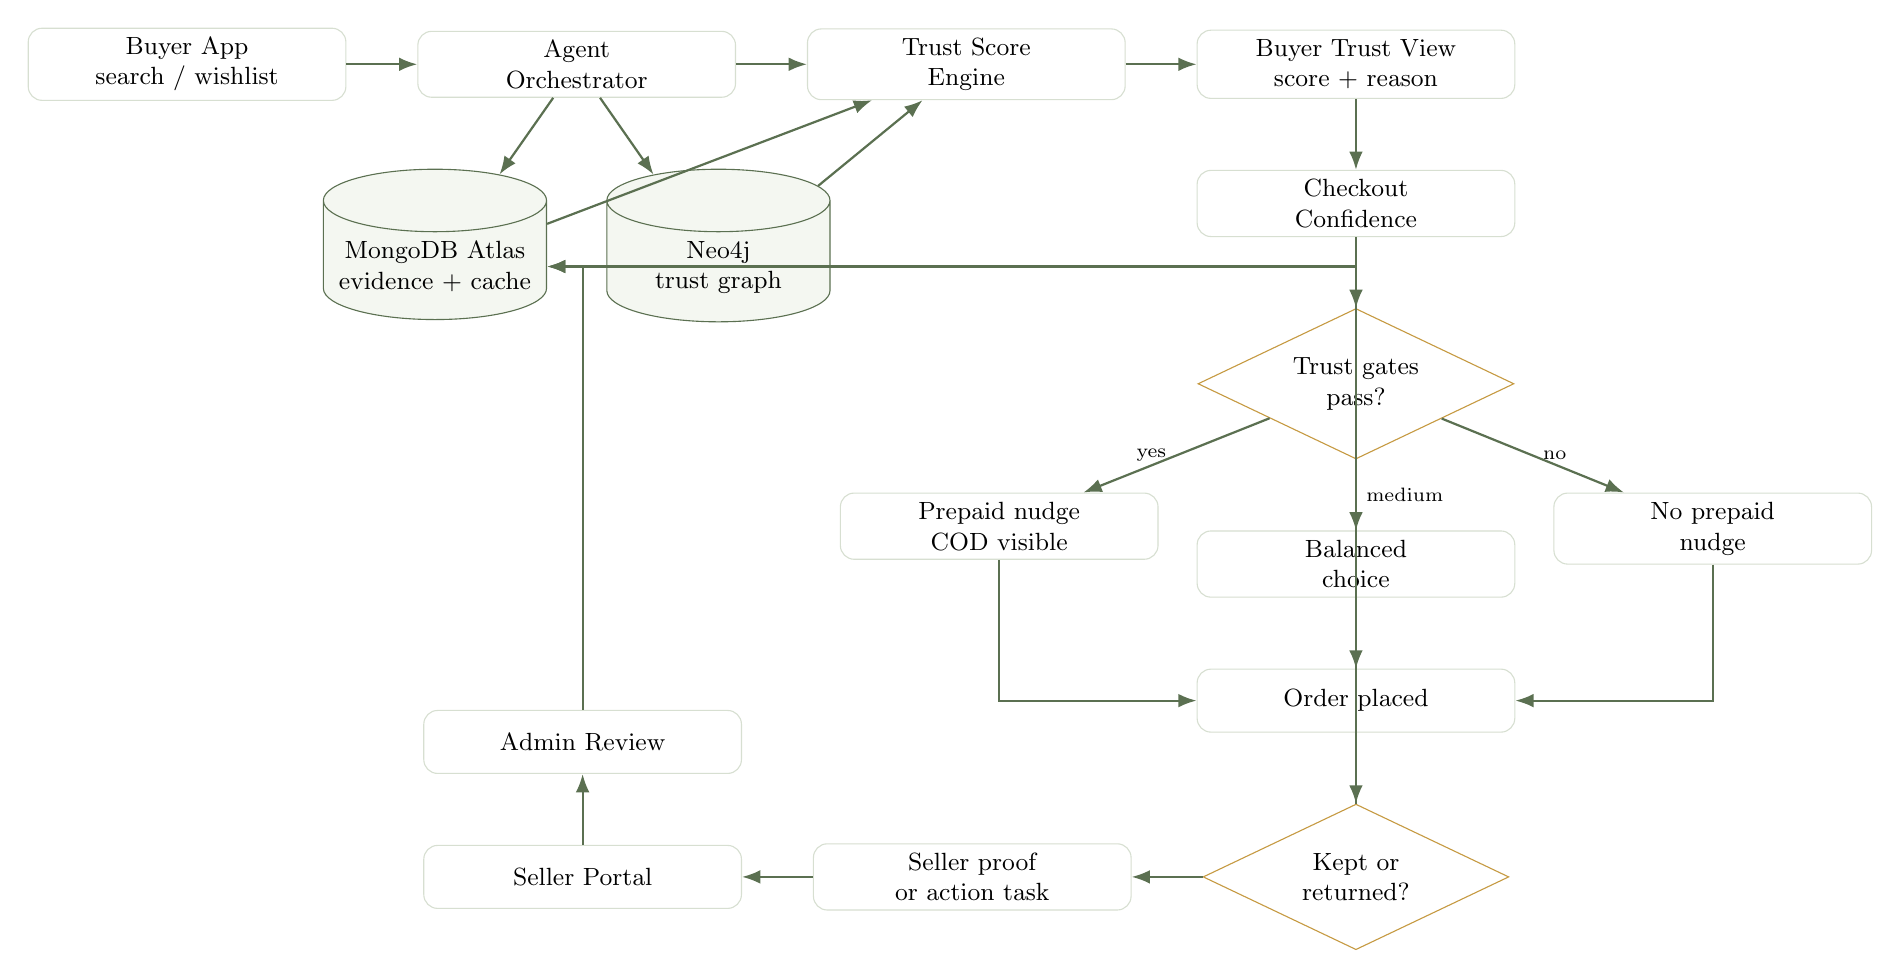
\begin{tikzpicture}[node distance=9mm and 9mm]
  \node[widebox] (buyer) {Buyer App\\search / wishlist};
  \node[widebox, right=of buyer] (agent) {Agent\\Orchestrator};
  \node[db, below=of agent, xshift=-18mm] (mongo) {MongoDB Atlas\\evidence + cache};
  \node[db, below=of agent, xshift=18mm] (neo) {Neo4j\\trust graph};
  \node[widebox, right=of agent] (score) {Trust Score\\Engine};
  \node[widebox, right=of score] (trust) {Buyer Trust View\\score + reason};
  \node[widebox, below=of trust] (checkout) {Checkout\\Confidence};
  \node[decision, below=of checkout] (gate) {Trust gates\\pass?};
  \node[widebox, below left=of gate, xshift=-6mm] (prepaid) {Prepaid nudge\\COD visible};
  \node[widebox, below=of gate] (balanced) {Balanced\\choice};
  \node[widebox, below right=of gate, xshift=6mm] (nonudge) {No prepaid\\nudge};
  \node[widebox, below=of balanced] (order) {Order placed};
  \node[decision, below=of order] (outcome) {Kept or\\returned?};
  \node[widebox, left=of outcome] (sellerTask) {Seller proof\\or action task};
  \node[widebox, left=of sellerTask] (seller) {Seller Portal};
  \node[widebox, above=of seller] (admin) {Admin Review};

  \draw[arrow] (buyer) -- (agent);
  \draw[arrow] (agent) -- (score);
  \draw[arrow] (agent) -- (mongo);
  \draw[arrow] (agent) -- (neo);
  \draw[arrow] (score) -- (trust);
  \draw[arrow] (trust) -- (checkout);
  \draw[arrow] (checkout) -- (gate);
  \draw[arrow] (gate) -- node[left,font=\scriptsize] {yes} (prepaid);
  \draw[arrow] (gate) -- node[right,font=\scriptsize] {medium} (balanced);
  \draw[arrow] (gate) -- node[right,font=\scriptsize] {no} (nonudge);
  \draw[arrow] (prepaid) |- (order);
  \draw[arrow] (balanced) -- (order);
  \draw[arrow] (nonudge) |- (order);
  \draw[arrow] (order) -- (outcome);
  \draw[arrow] (outcome) -- (sellerTask);
  \draw[arrow] (sellerTask) -- (seller);
  \draw[arrow] (seller) -- (admin);
  \draw[arrow] (admin) |- (mongo);
  \draw[arrow] (outcome) |- (mongo);
  \draw[arrow] (mongo) -- (score);
  \draw[arrow] (neo) -- (score);
\end{tikzpicture}
\end{center}

\subsection{17.2 Buyer Flow}
\begin{center}
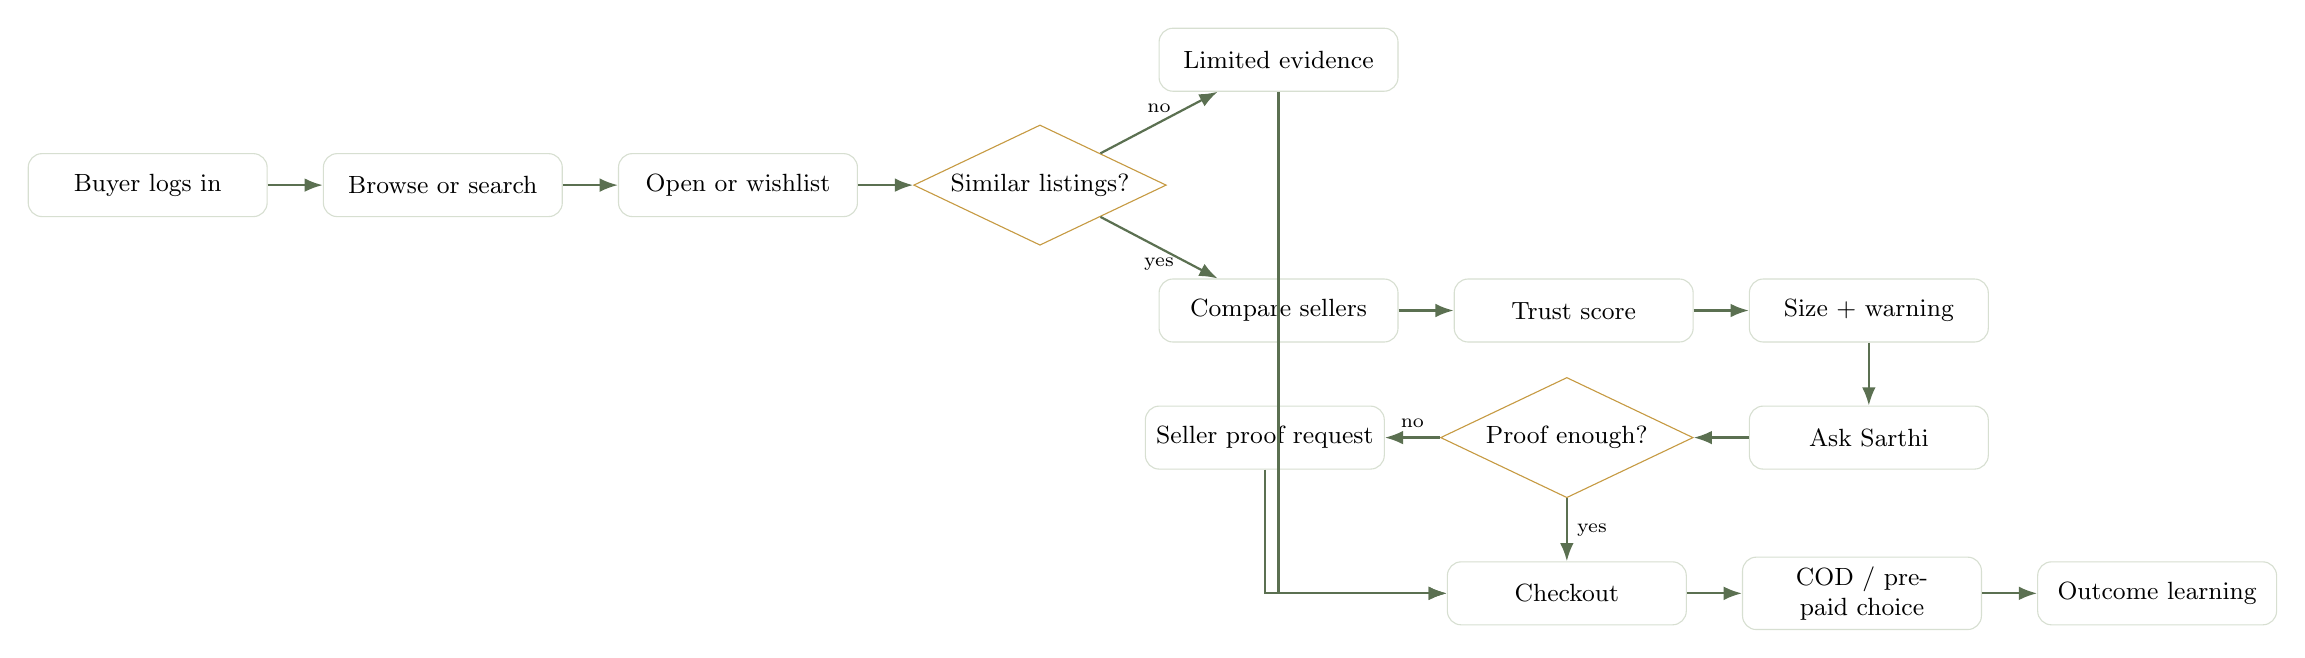
\begin{tikzpicture}[node distance=8mm and 7mm]
  \node[box] (login) {Buyer logs in};
  \node[box, right=of login] (browse) {Browse or search};
  \node[box, right=of browse] (select) {Open or wishlist};
  \node[decision, right=of select] (similar) {Similar listings?};
  \node[box, above right=of similar] (limited) {Limited evidence};
  \node[box, below right=of similar] (compare) {Compare sellers};
  \node[box, right=of compare] (score) {Trust score};
  \node[box, right=of score] (detail) {Size + warning};
  \node[box, below=of detail] (ask) {Ask Sarthi};
  \node[decision, left=of ask] (proof) {Proof enough?};
  \node[box, left=of proof] (request) {Seller proof request};
  \node[box, below=of proof] (checkout) {Checkout};
  \node[box, right=of checkout] (payment) {COD / prepaid choice};
  \node[box, right=of payment] (learn) {Outcome learning};

  \draw[arrow] (login) -- (browse);
  \draw[arrow] (browse) -- (select);
  \draw[arrow] (select) -- (similar);
  \draw[arrow] (similar) -- node[above,font=\scriptsize] {no} (limited);
  \draw[arrow] (similar) -- node[below,font=\scriptsize] {yes} (compare);
  \draw[arrow] (compare) -- (score);
  \draw[arrow] (score) -- (detail);
  \draw[arrow] (detail) -- (ask);
  \draw[arrow] (ask) -- (proof);
  \draw[arrow] (proof) -- node[above,font=\scriptsize] {no} (request);
  \draw[arrow] (proof) -- node[right,font=\scriptsize] {yes} (checkout);
  \draw[arrow] (limited) |- (checkout);
  \draw[arrow] (request) |- (checkout);
  \draw[arrow] (checkout) -- (payment);
  \draw[arrow] (payment) -- (learn);
\end{tikzpicture}
\end{center}

\subsection{17.3 Seller And Admin Flow}
\begin{center}
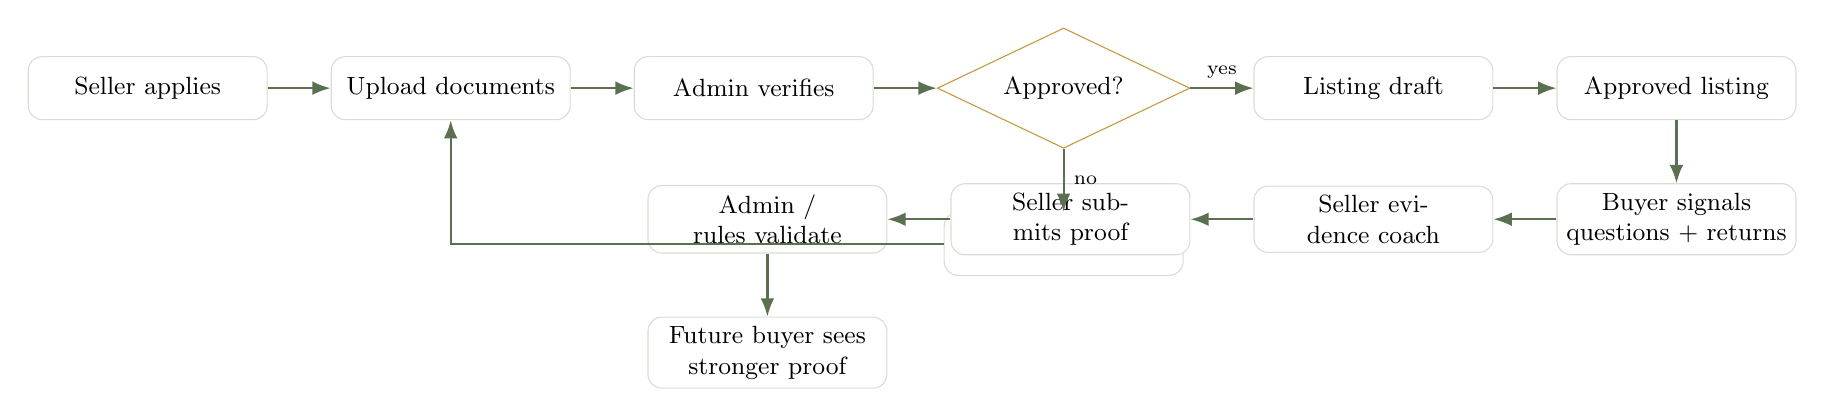
\begin{tikzpicture}[node distance=8mm and 8mm]
  \node[box] (apply) {Seller applies};
  \node[box, right=of apply] (docs) {Upload documents};
  \node[box, right=of docs] (review) {Admin verifies};
  \node[decision, right=of review] (approved) {Approved?};
  \node[box, below=of approved] (revision) {Revision};
  \node[box, right=of approved] (draft) {Listing draft};
  \node[box, right=of draft] (publish) {Approved listing};
  \node[box, below=of publish] (signals) {Buyer signals\\questions + returns};
  \node[box, left=of signals] (coach) {Seller evidence coach};
  \node[box, left=of coach] (proof) {Seller submits proof};
  \node[box, left=of proof] (validate) {Admin / rules validate};
  \node[box, below=of validate] (future) {Future buyer sees\\stronger proof};

  \draw[arrow] (apply) -- (docs);
  \draw[arrow] (docs) -- (review);
  \draw[arrow] (review) -- (approved);
  \draw[arrow] (approved) -- node[above,font=\scriptsize] {yes} (draft);
  \draw[arrow] (approved) -- node[right,font=\scriptsize] {no} (revision);
  \draw[arrow] (revision) -| (docs);
  \draw[arrow] (draft) -- (publish);
  \draw[arrow] (publish) -- (signals);
  \draw[arrow] (signals) -- (coach);
  \draw[arrow] (coach) -- (proof);
  \draw[arrow] (proof) -- (validate);
  \draw[arrow] (validate) -- (future);
\end{tikzpicture}
\end{center}

\section{18. Final Summary}
Sarthi is a closed-loop trust product. It starts with buyer confusion, calculates explainable trust, supports safer checkout decisions, sends aggregate proof gaps to sellers, uses admin review for governance, and learns from delivery outcomes.

\end{document}
